\documentclass[twoside]{book}

% Packages required by doxygen
\usepackage{fixltx2e}
\usepackage{calc}
\usepackage{doxygen}
\usepackage[export]{adjustbox} % also loads graphicx
\usepackage{graphicx}
\usepackage[utf8]{inputenc}
\usepackage{makeidx}
\usepackage{multicol}
\usepackage{multirow}
\PassOptionsToPackage{warn}{textcomp}
\usepackage{textcomp}
\usepackage[nointegrals]{wasysym}
\usepackage[table]{xcolor}

% Font selection
\usepackage[T1]{fontenc}
\usepackage[scaled=.90]{helvet}
\usepackage{courier}
\usepackage{amssymb}
\usepackage{sectsty}
\renewcommand{\familydefault}{\sfdefault}
\allsectionsfont{%
  \fontseries{bc}\selectfont%
  \color{darkgray}%
}
\renewcommand{\DoxyLabelFont}{%
  \fontseries{bc}\selectfont%
  \color{darkgray}%
}
\newcommand{\+}{\discretionary{\mbox{\scriptsize$\hookleftarrow$}}{}{}}

% Page & text layout
\usepackage{geometry}
\geometry{%
  a4paper,%
  top=2.5cm,%
  bottom=2.5cm,%
  left=2.5cm,%
  right=2.5cm%
}
\tolerance=750
\hfuzz=15pt
\hbadness=750
\setlength{\emergencystretch}{15pt}
\setlength{\parindent}{0cm}
\setlength{\parskip}{3ex plus 2ex minus 2ex}
\makeatletter
\renewcommand{\paragraph}{%
  \@startsection{paragraph}{4}{0ex}{-1.0ex}{1.0ex}{%
    \normalfont\normalsize\bfseries\SS@parafont%
  }%
}
\renewcommand{\subparagraph}{%
  \@startsection{subparagraph}{5}{0ex}{-1.0ex}{1.0ex}{%
    \normalfont\normalsize\bfseries\SS@subparafont%
  }%
}
\makeatother

% Headers & footers
\usepackage{fancyhdr}
\pagestyle{fancyplain}
\fancyhead[LE]{\fancyplain{}{\bfseries\thepage}}
\fancyhead[CE]{\fancyplain{}{}}
\fancyhead[RE]{\fancyplain{}{\bfseries\leftmark}}
\fancyhead[LO]{\fancyplain{}{\bfseries\rightmark}}
\fancyhead[CO]{\fancyplain{}{}}
\fancyhead[RO]{\fancyplain{}{\bfseries\thepage}}
\fancyfoot[LE]{\fancyplain{}{}}
\fancyfoot[CE]{\fancyplain{}{}}
\fancyfoot[RE]{\fancyplain{}{\bfseries\scriptsize Generated by Doxygen }}
\fancyfoot[LO]{\fancyplain{}{\bfseries\scriptsize Generated by Doxygen }}
\fancyfoot[CO]{\fancyplain{}{}}
\fancyfoot[RO]{\fancyplain{}{}}
\renewcommand{\footrulewidth}{0.4pt}
\renewcommand{\chaptermark}[1]{%
  \markboth{#1}{}%
}
\renewcommand{\sectionmark}[1]{%
  \markright{\thesection\ #1}%
}

% Indices & bibliography
\usepackage{natbib}
\usepackage[titles]{tocloft}
\setcounter{tocdepth}{3}
\setcounter{secnumdepth}{5}
\makeindex

% Hyperlinks (required, but should be loaded last)
\usepackage{ifpdf}
\ifpdf
  \usepackage[pdftex,pagebackref=true]{hyperref}
\else
  \usepackage[ps2pdf,pagebackref=true]{hyperref}
\fi
\hypersetup{%
  colorlinks=true,%
  linkcolor=blue,%
  citecolor=blue,%
  unicode%
}

% Custom commands
\newcommand{\clearemptydoublepage}{%
  \newpage{\pagestyle{empty}\cleardoublepage}%
}

\usepackage{caption}
\captionsetup{labelsep=space,justification=centering,font={bf},singlelinecheck=off,skip=4pt,position=top}

%===== C O N T E N T S =====

\begin{document}

% Titlepage & ToC
\hypersetup{pageanchor=false,
             bookmarksnumbered=true,
             pdfencoding=unicode
            }
\pagenumbering{alph}
\begin{titlepage}
\vspace*{7cm}
\begin{center}%
{\Large Human Obstacle Detector and Tracker }\\
\vspace*{1cm}
{\large Generated by Doxygen 1.8.13}\\
\end{center}
\end{titlepage}
\clearemptydoublepage
\pagenumbering{roman}
\tableofcontents
\clearemptydoublepage
\pagenumbering{arabic}
\hypersetup{pageanchor=true}

%--- Begin generated contents ---
\chapter{Class Index}
\section{Class List}
Here are the classes, structs, unions and interfaces with brief descriptions\+:\begin{DoxyCompactList}
\item\contentsline{section}{\hyperlink{structCentroid}{Centroid} }{\pageref{structCentroid}}{}
\item\contentsline{section}{\hyperlink{classData}{Data$<$ T $>$} \\*Wrapper class for any encapsulate any datatype object }{\pageref{classData}}{}
\item\contentsline{section}{\hyperlink{classDataReader}{Data\+Reader$<$ T, U $>$} \\*Generic datareader class }{\pageref{classDataReader}}{}
\item\contentsline{section}{\hyperlink{classDetector}{Detector} \\*Generic object detection class }{\pageref{classDetector}}{}
\item\contentsline{section}{\hyperlink{classDriver}{Driver} \\*This class is responsible for executing the complete detection pipline }{\pageref{classDriver}}{}
\item\contentsline{section}{\hyperlink{classFrameTransformation}{Frame\+Transformation} \\*Class responsible to convert the coordinates from camera frame to robot frame }{\pageref{classFrameTransformation}}{}
\item\contentsline{section}{\hyperlink{classHumanDetector}{Human\+Detector} }{\pageref{classHumanDetector}}{}
\item\contentsline{section}{\hyperlink{classImageReader}{Image\+Reader} }{\pageref{classImageReader}}{}
\item\contentsline{section}{\hyperlink{classModel}{Model$<$ T, U $>$} \\*Abstract \hyperlink{classModel}{Model} class for all the ML models }{\pageref{classModel}}{}
\item\contentsline{section}{\hyperlink{classPreProcessor}{Pre\+Processor} \\*Class to do all the preprocessing of the data }{\pageref{classPreProcessor}}{}
\item\contentsline{section}{\hyperlink{classSVMHumanClassifier}{S\+V\+M\+Human\+Classifier} }{\pageref{classSVMHumanClassifier}}{}
\end{DoxyCompactList}

\chapter{Class Documentation}
\hypertarget{classDetector}{}\section{Detector Class Reference}
\label{classDetector}\index{Detector@{Detector}}


Generic object detection class.  




{\ttfamily \#include $<$detector.\+hpp$>$}



Inheritance diagram for Detector\+:\nopagebreak
\begin{figure}[H]
\begin{center}
\leavevmode
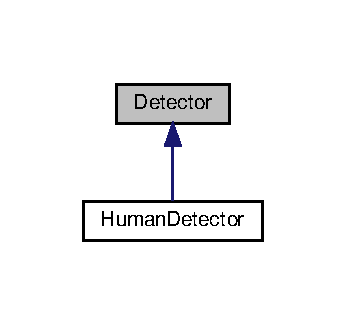
\includegraphics[width=166pt]{classDetector__inherit__graph}
\end{center}
\end{figure}
\subsection*{Public Member Functions}
\begin{DoxyCompactItemize}
\item 
\mbox{\Hypertarget{classDetector_afdf99890fb93a11252eef0dd85598c15}\label{classDetector_afdf99890fb93a11252eef0dd85598c15}} 
virtual std\+::vector$<$ Coord3D $>$ \hyperlink{classDetector_afdf99890fb93a11252eef0dd85598c15}{detect} (const cv\+::\+Mat \&input\+Data, bool is\+Test\+Mode)=0
\begin{DoxyCompactList}\small\item\em detects objects in image \end{DoxyCompactList}\item 
\mbox{\Hypertarget{classDetector_afaaefdcb9f6271dadf13fd2158e5d9be}\label{classDetector_afaaefdcb9f6271dadf13fd2158e5d9be}} 
virtual double {\bfseries evaluate\+Model} (const cv\+::\+Mat \&input\+Data, std\+::vector$<$ \hyperlink{structCentroid}{Centroid} $>$ gt\+\_\+centroids)=0
\end{DoxyCompactItemize}


\subsection{Detailed Description}
Generic object detection class. 

The documentation for this class was generated from the following file\+:\begin{DoxyCompactItemize}
\item 
include/\hyperlink{detector_8hpp}{detector.\+hpp}\end{DoxyCompactItemize}

%--- End generated contents ---

% Index
\backmatter
\newpage
\phantomsection
\clearemptydoublepage
\addcontentsline{toc}{chapter}{Index}
\printindex

\end{document}
